\section{Benchmarking of Planners}
In the previous sections, we found out the path plans for optimal welding using the 2Dof rotary table. We also addressed the problem of reachability and showed how it can be overcome using the table. In this chapter we will delve into the effects that the table has on the motion planners, in terms of time taken to generate a plan, correctness of solution generated and memory consumed while doing so. We consider 2 different scenarios, for benchmarking the planners first without optimizing the table position and next with the table optimization turned on. The results show a remarkable improvement, in terms of both time and valid solution generation when table optimization is used. The use cases are illustrated in figures (\ref{bm:uc1} and \ref{bm:uc2}).
The configuration details of the planners are presented in the appendix section.
\begin{figure}[!htbp] %  figure placement: here, top, bottom, or page
	\centering
	\begin{subfigure}[b]{0.4\textwidth}
		\frame{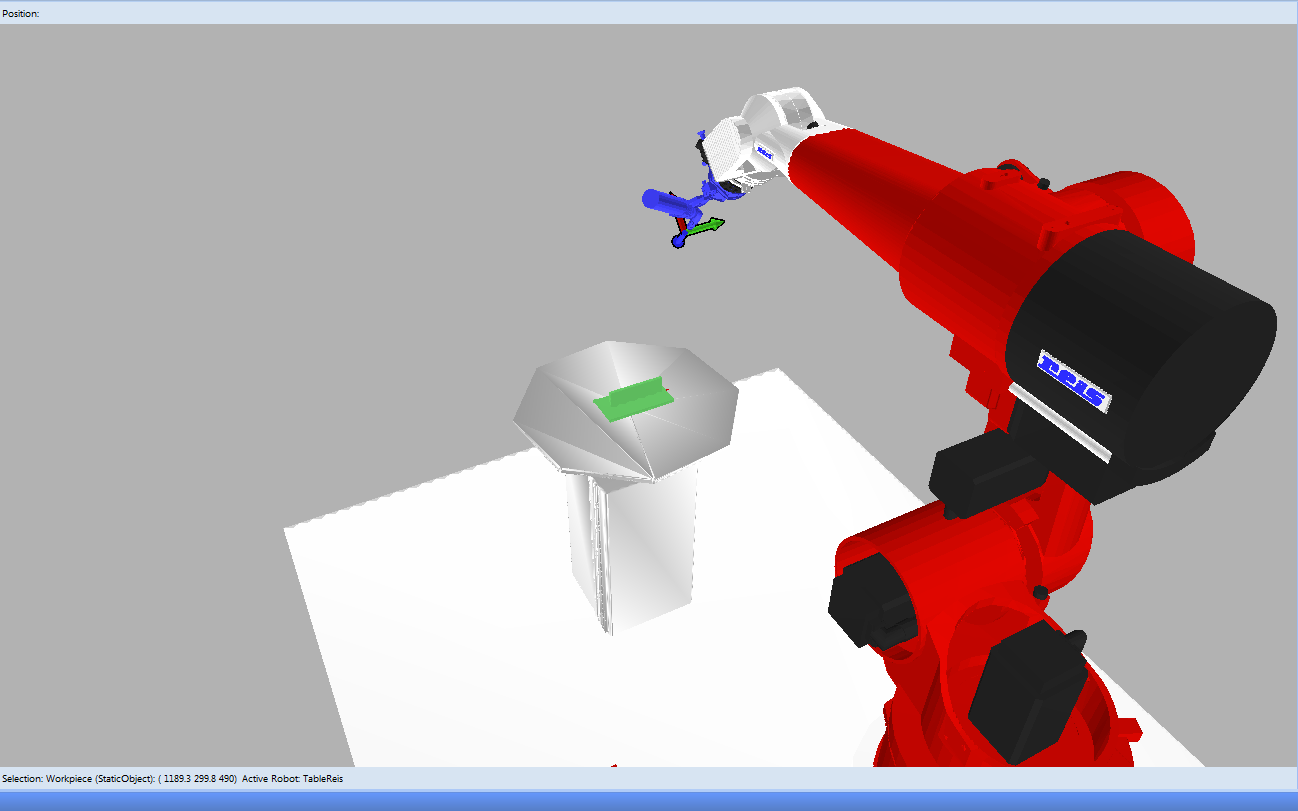
\includegraphics[width=1\textwidth,height=0.2\textheight]{images/un_opt_bnch.png}}
		\caption{Use Case Without Table Position Optimization}  
		\label{bm:uc1}
	\end{subfigure}
	\begin{subfigure}[b]{0.4\textwidth}
		\frame{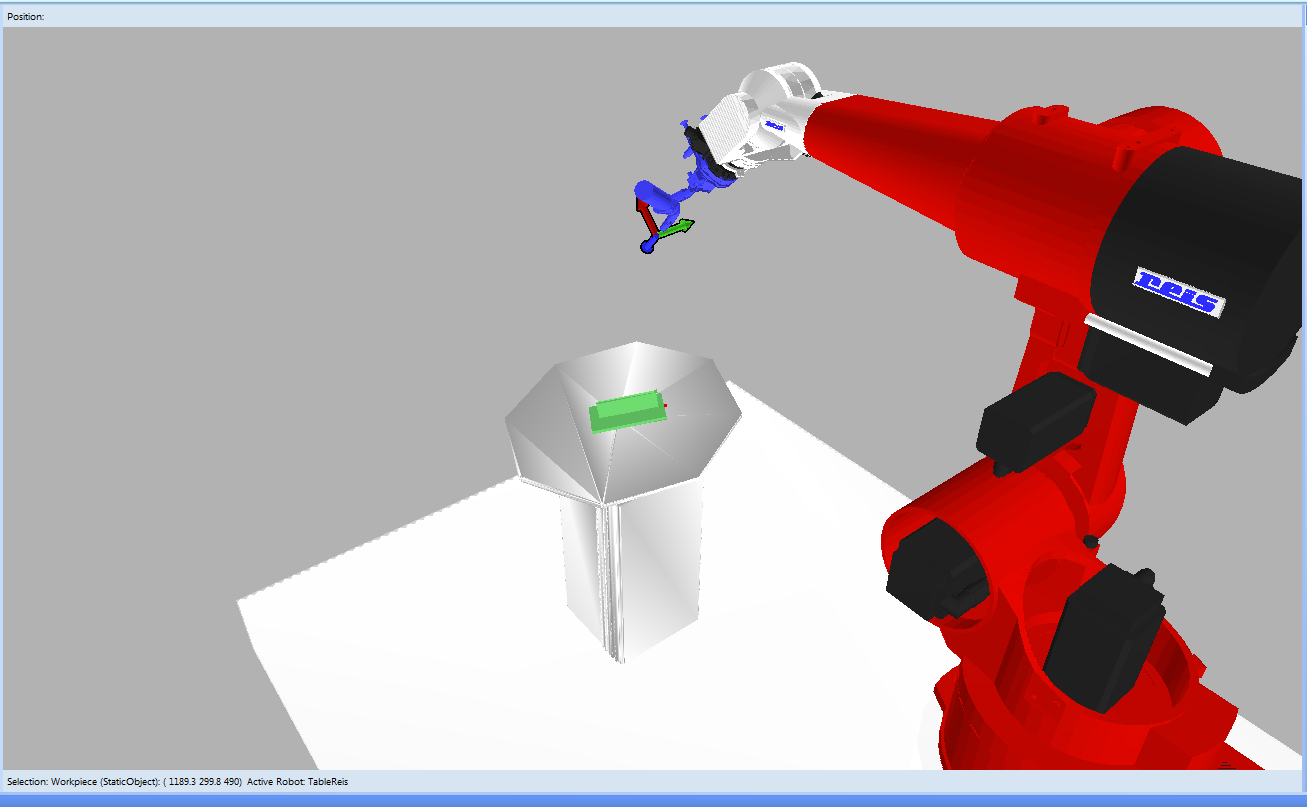
\includegraphics[width=1\textwidth,height=0.2\textheight]{images/opt_bnch.png}}
		\caption{Use Case With Table Position Optimization}  
		\label{bm:uc2}
	\end{subfigure}	
	\caption{Benchmarking Use Cases}
	\label{bm:uc}
\end{figure}

\begin{figure}[!ht] %  figure placement: here, top, bottom, or page
	\centering
	\frame{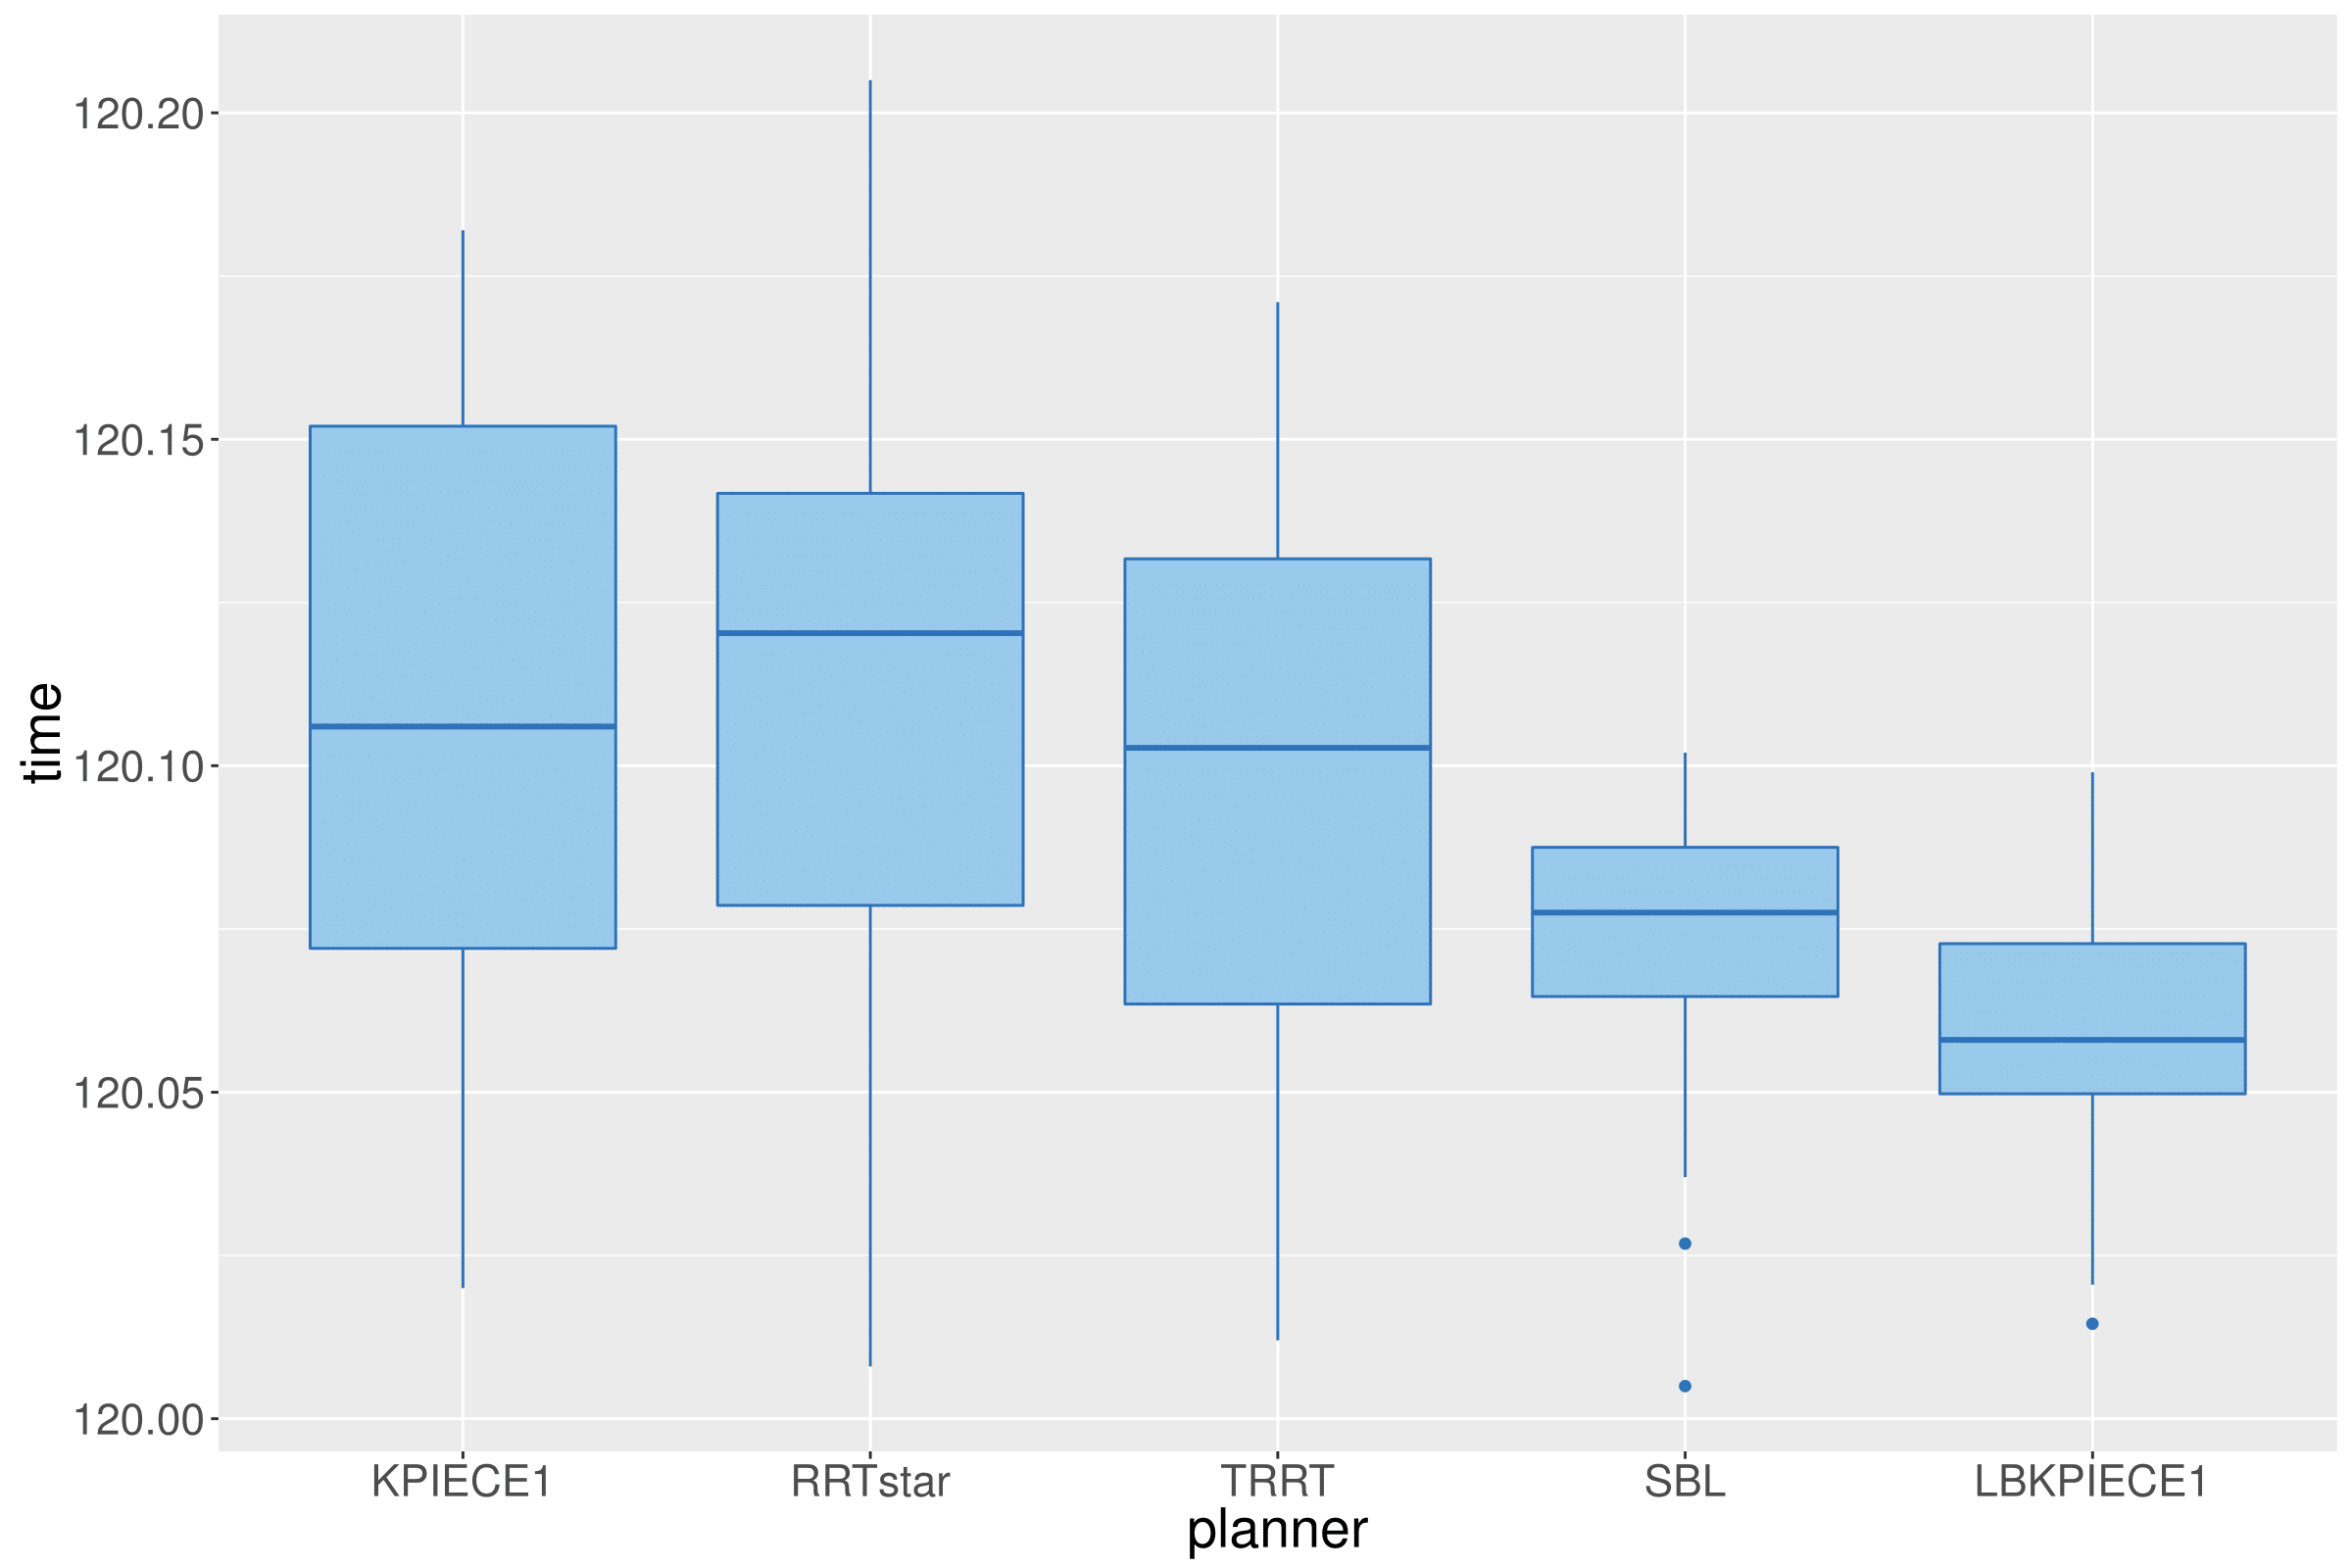
\includegraphics[width=0.8\textwidth,scale=0.6]{images/norm_time-1.png}}
	\caption{Time Consumed for Unoptimized Motion Planning }
	\label{fig:bm1}
\end{figure}
\begin{figure}[!ht] %  figure placement: here, top, bottom, or page
	\centering
	\frame{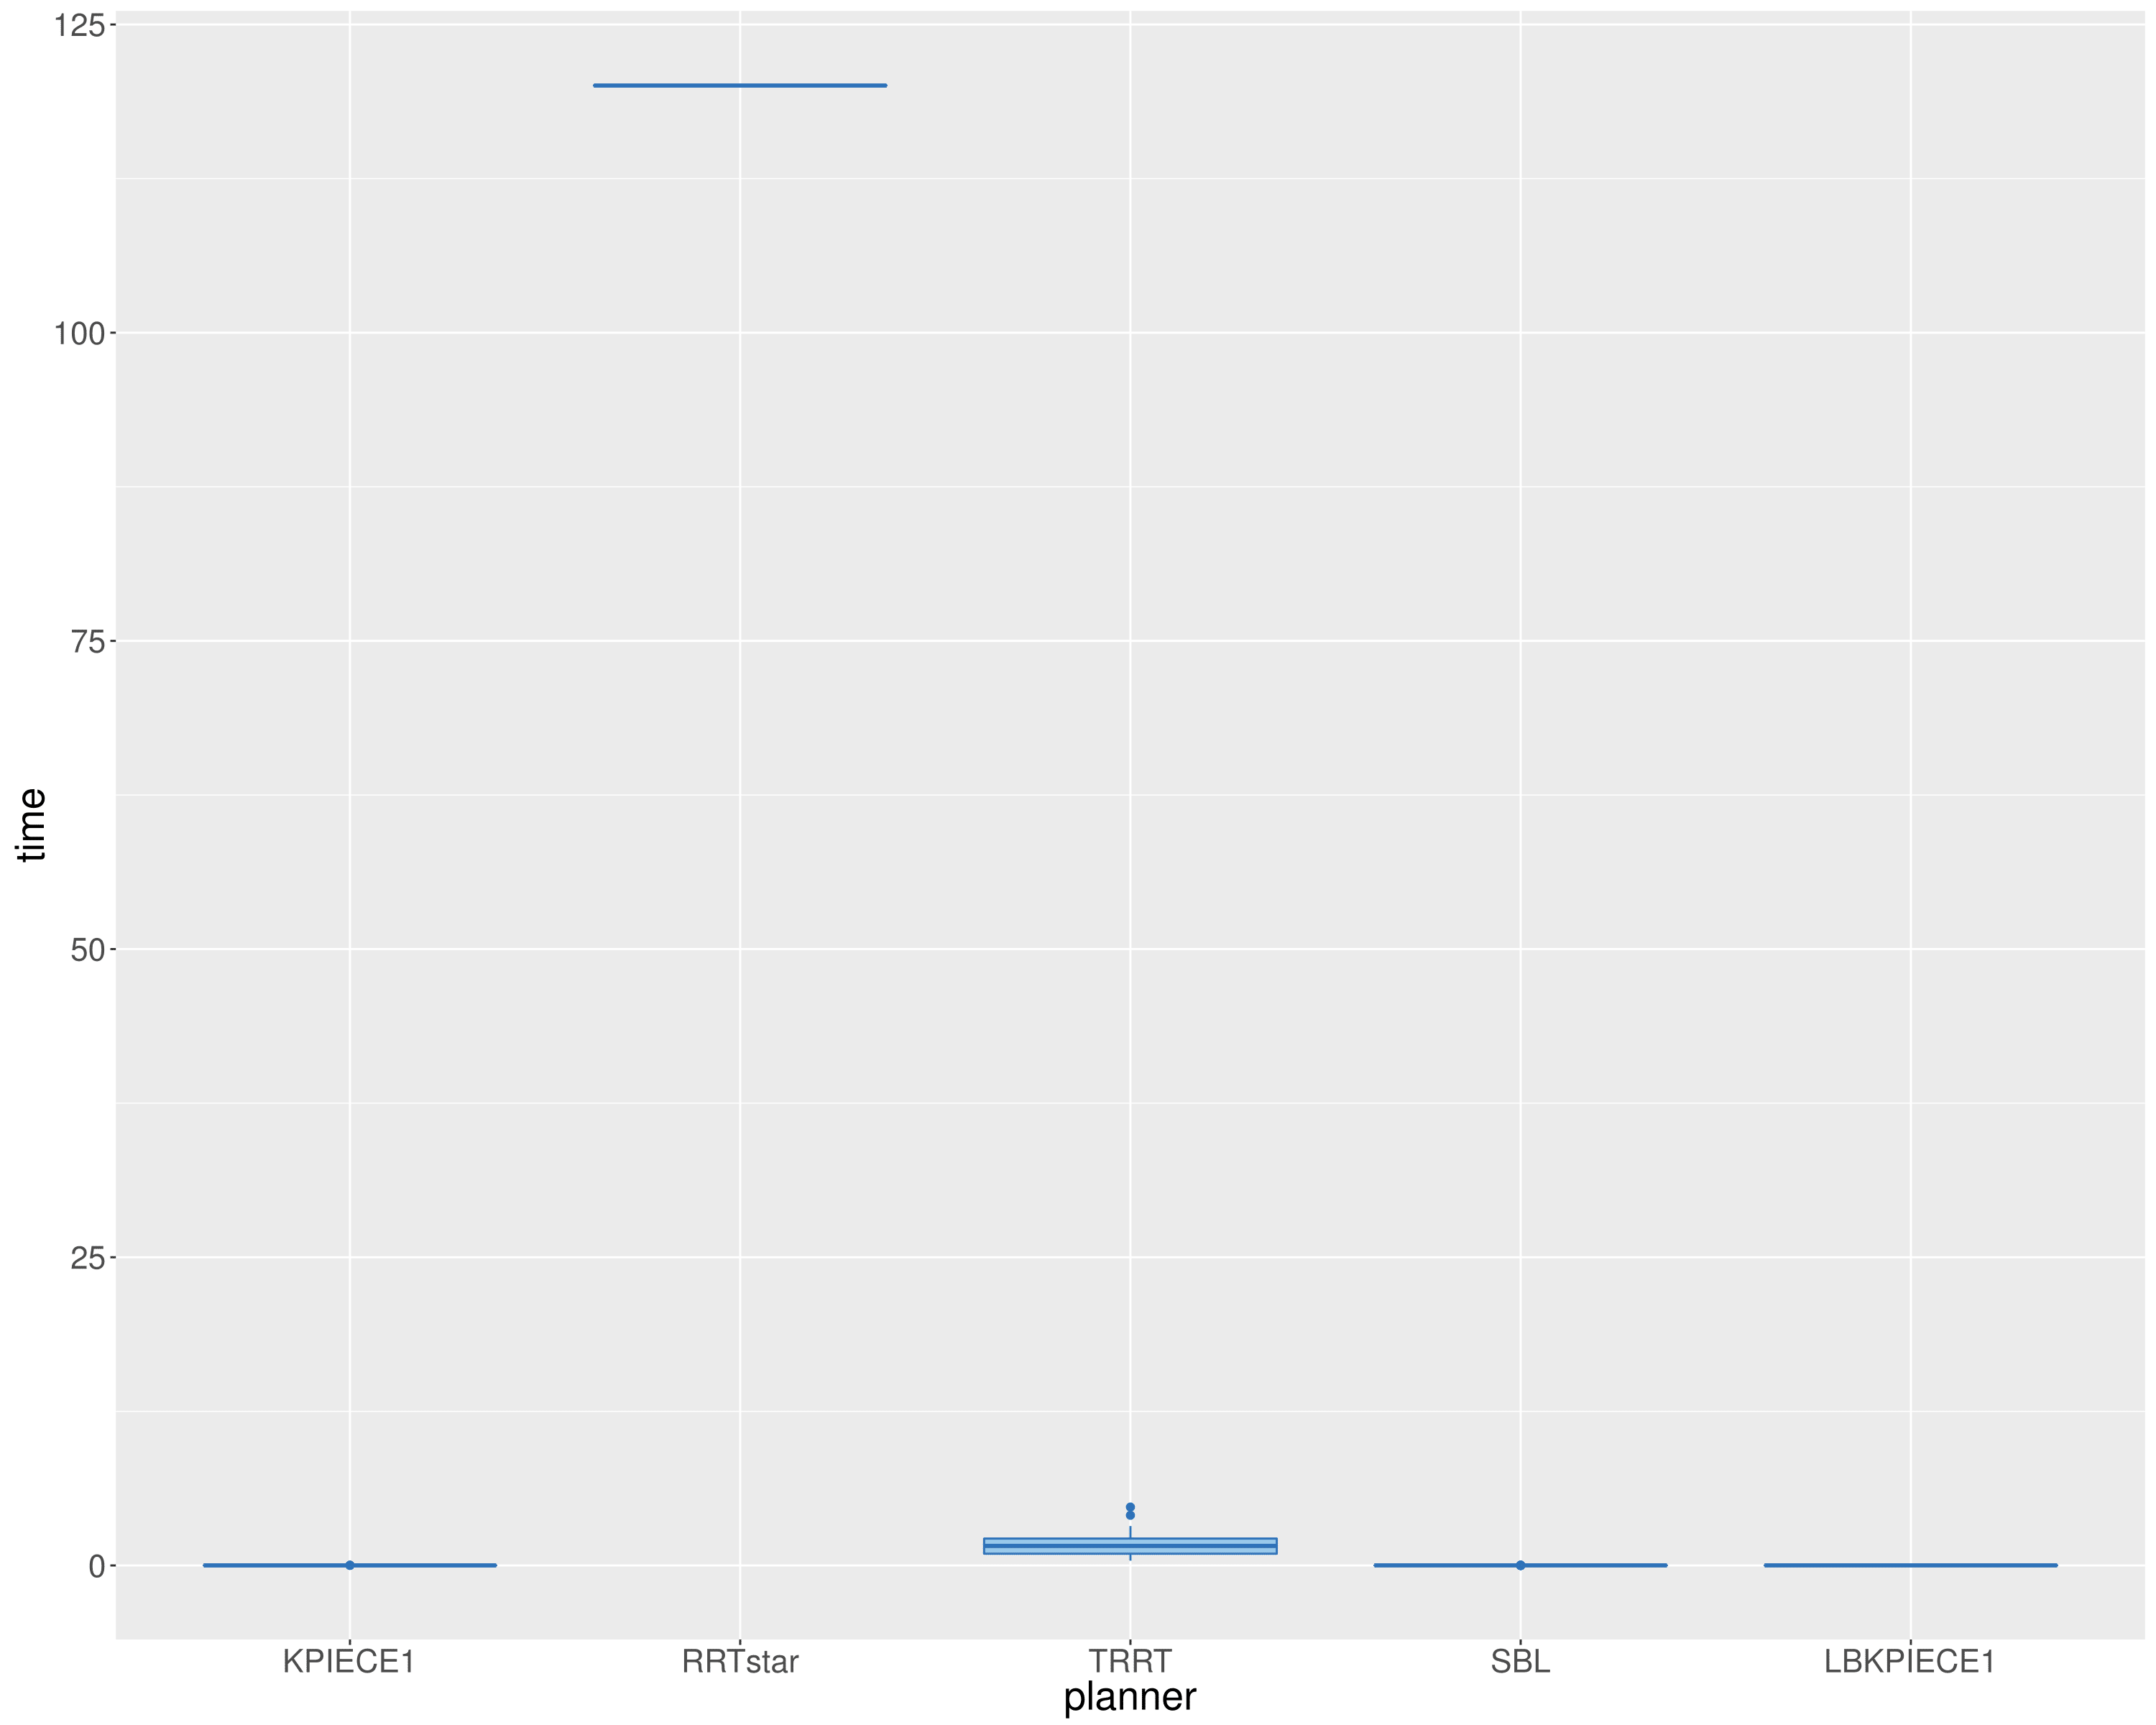
\includegraphics[width=0.8\textwidth,scale=0.6]{images/opt_time-1.png}}
	\caption{Time Consumed for Optimized Motion Planning with Table}
	\label{fig:bm2}
\end{figure}
\begin{figure}[!ht] %  figure placement: here, top, bottom, or page
	\centering
	\frame{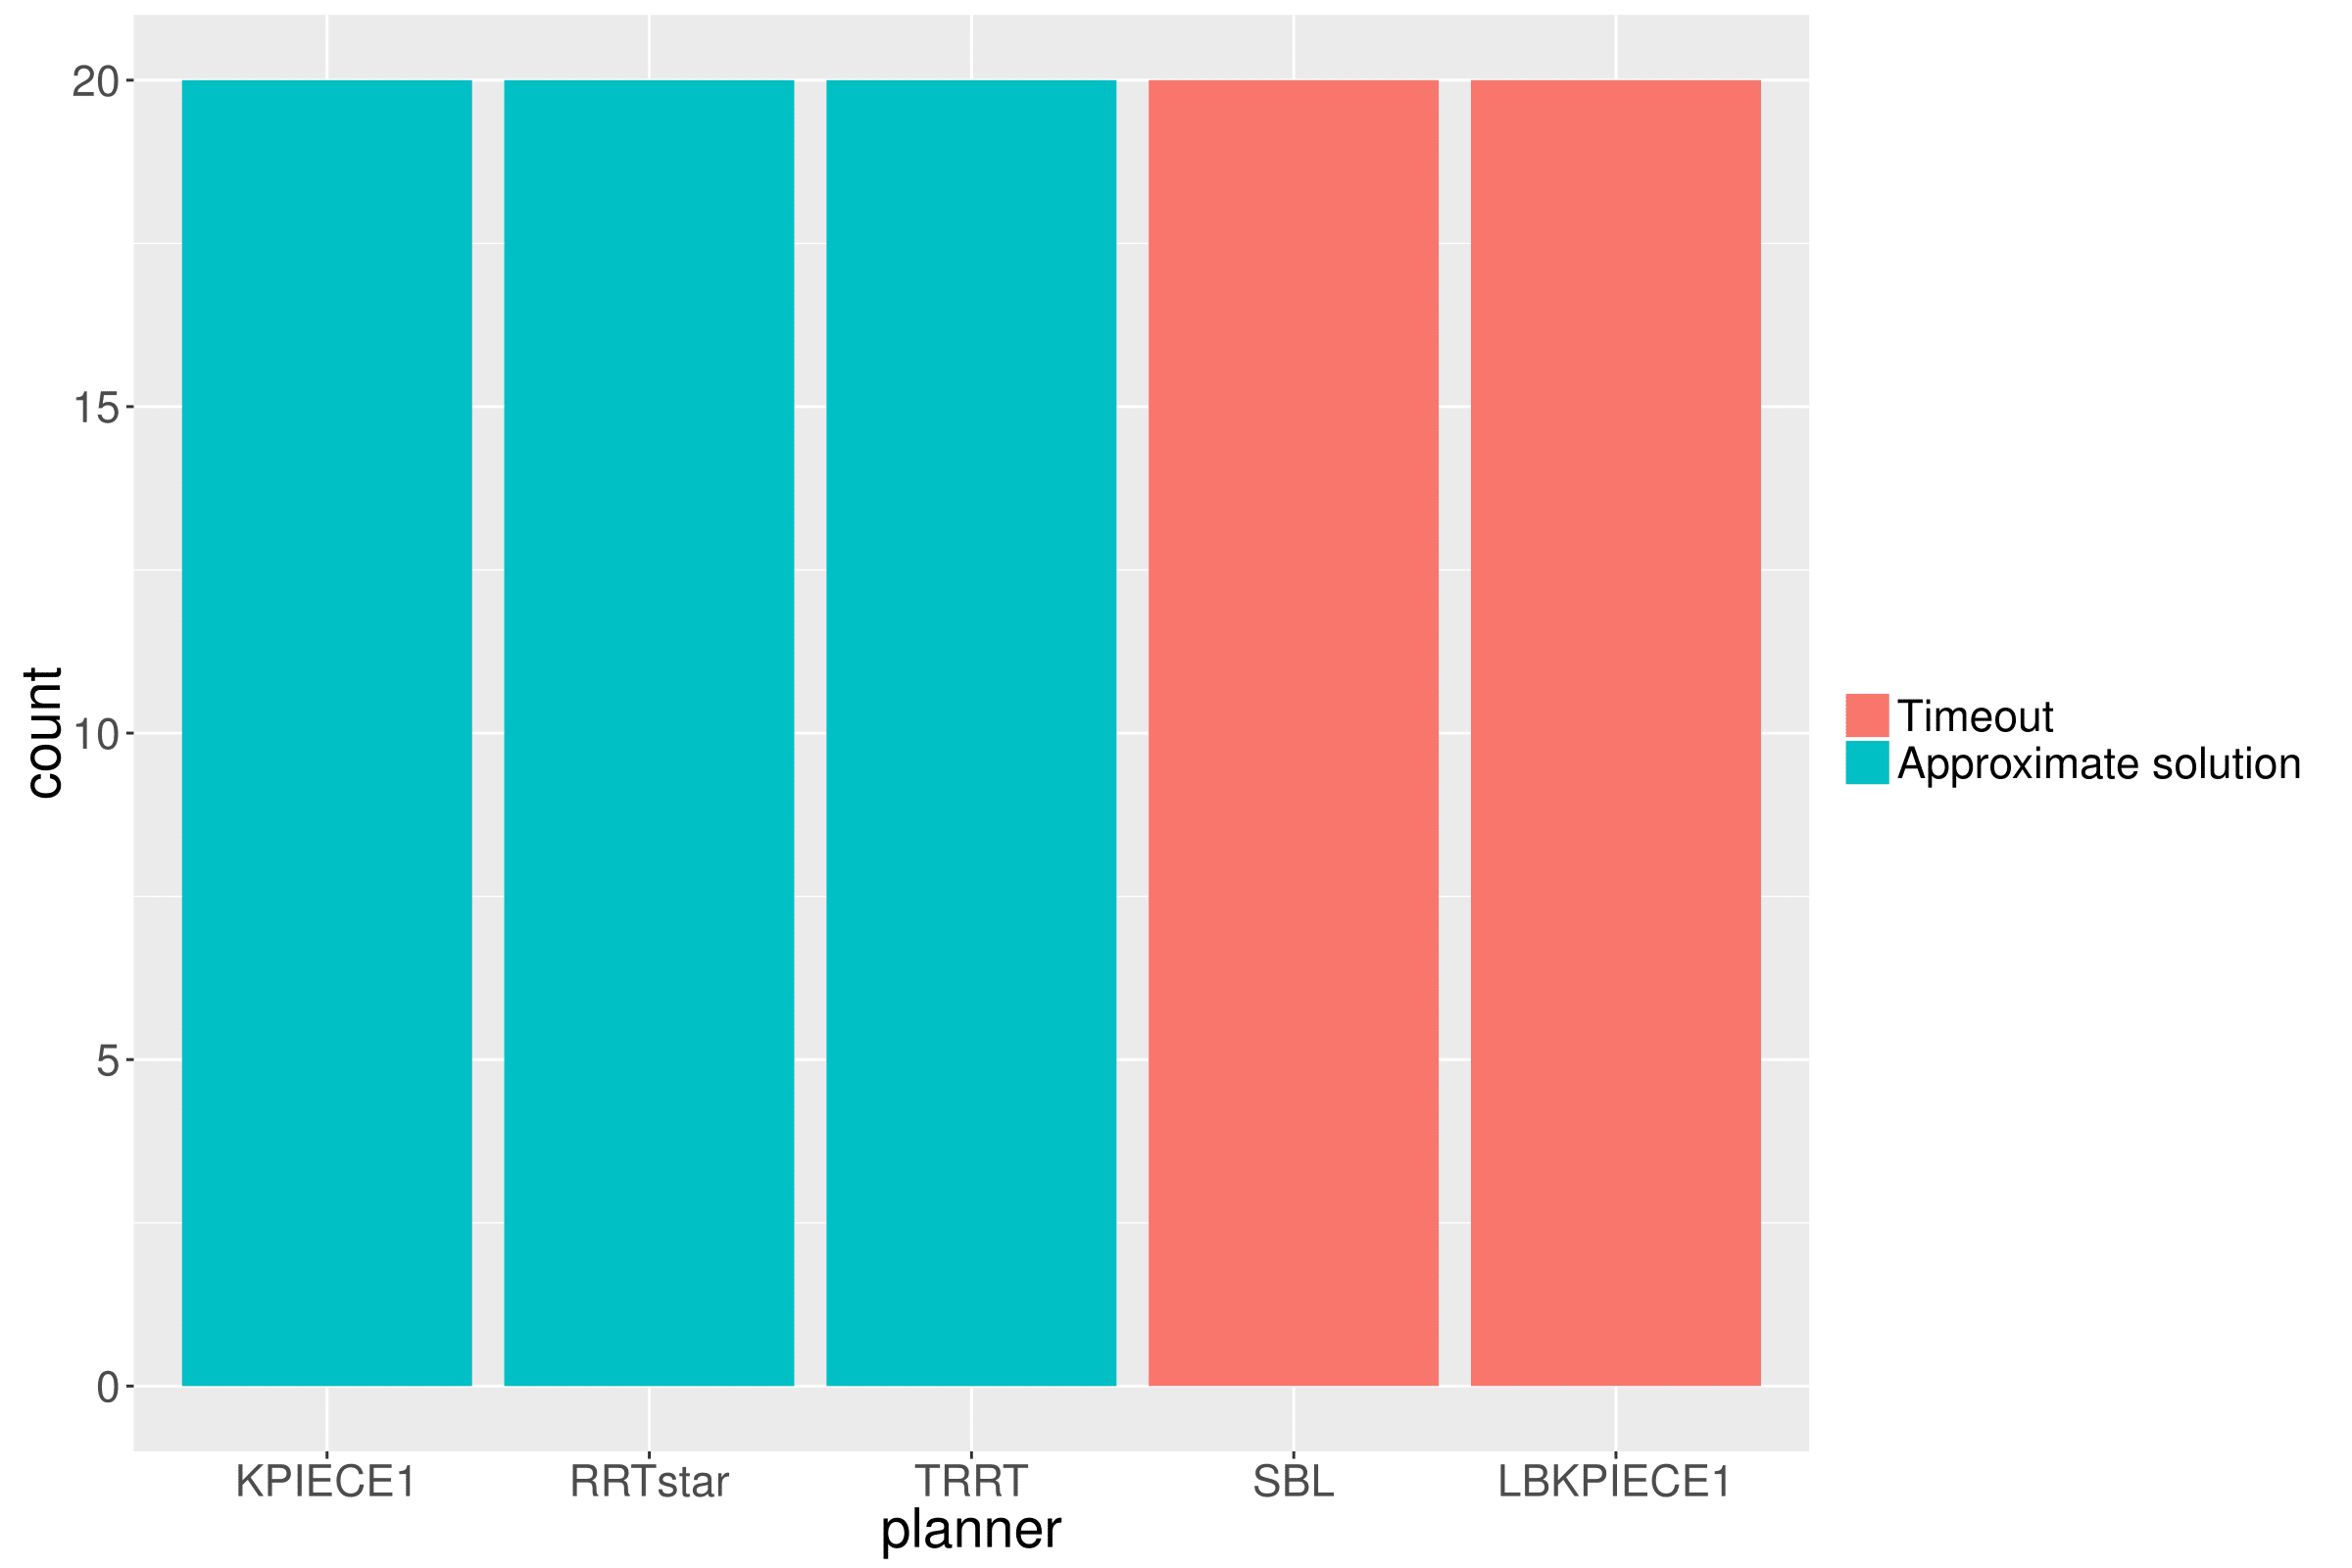
\includegraphics[width=0.8\textwidth,scale=0.6]{images/norm_status-1.png}}
	\caption{Status of Motion Planning: Unoptimized}
	\label{fig:bm3}
\end{figure}
\begin{figure}[!ht] %  figure placement: here, top, bottom, or page
	\centering
	\frame{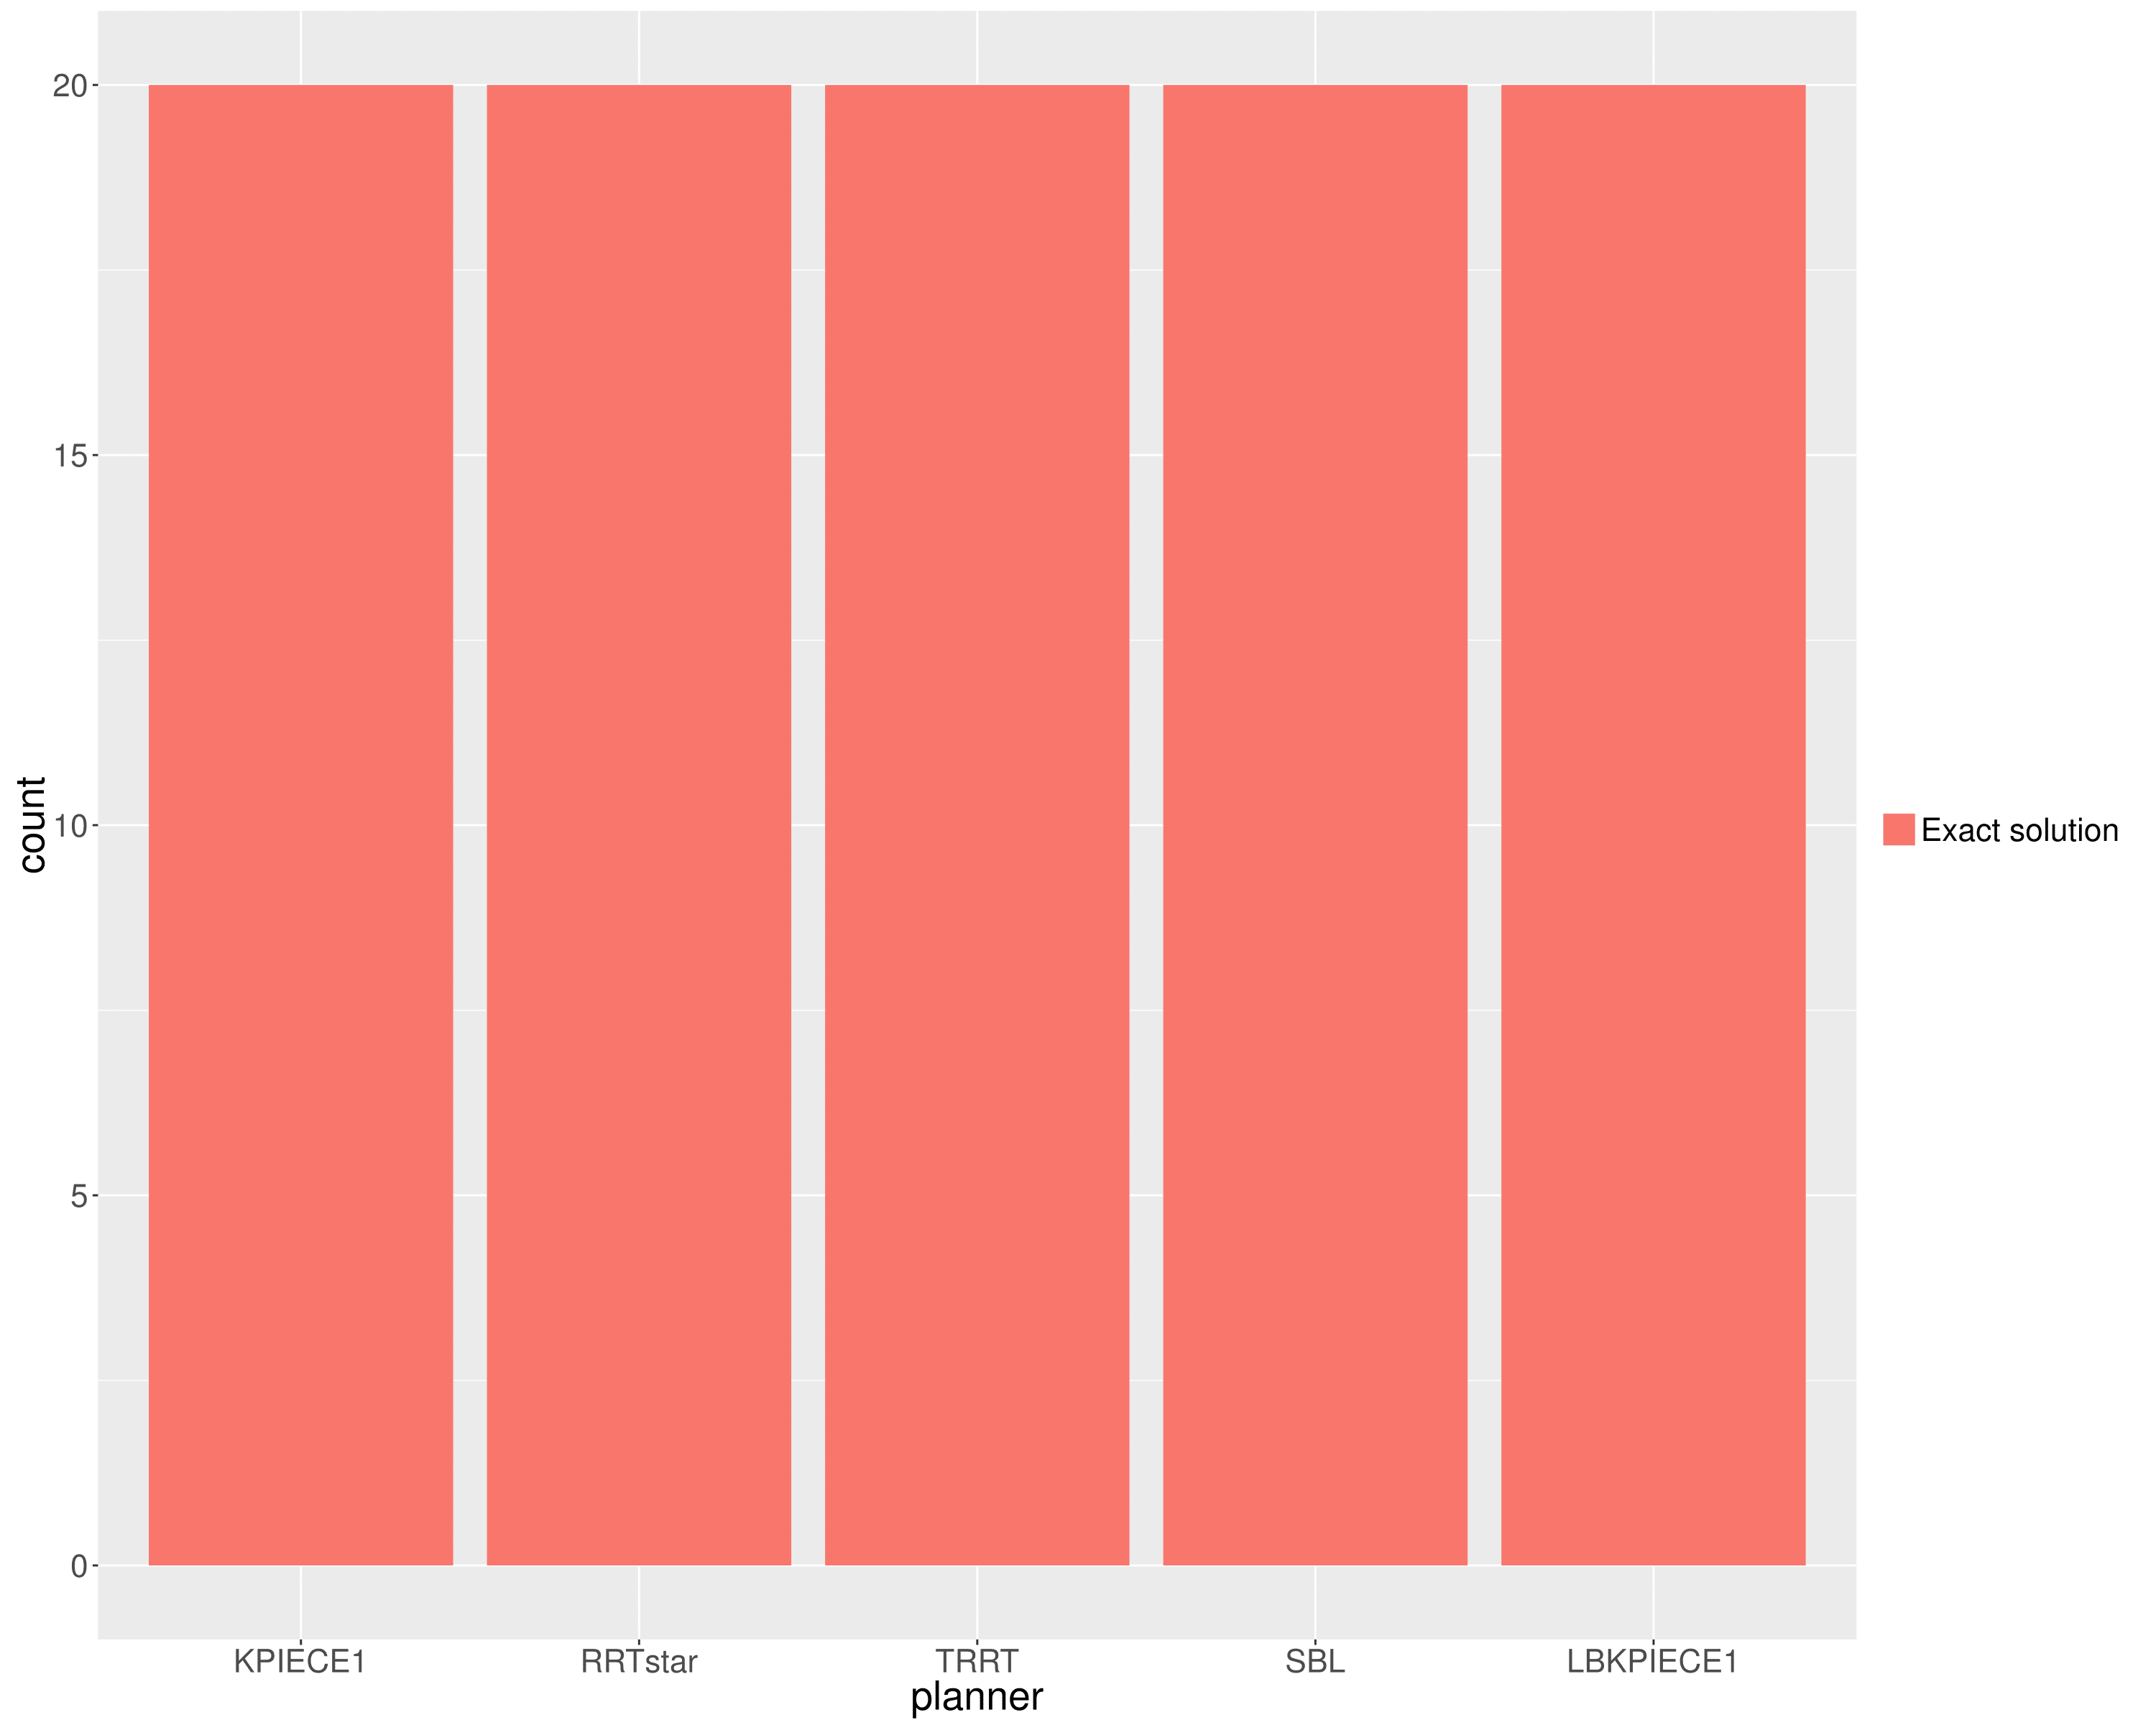
\includegraphics[width=0.8\textwidth,scale=0.6]{images/opt_status-1.png}}
	\caption{Status of Motion Planning:Using Table Optimization}
	\label{fig:bm4}
\end{figure}
\begin{figure}[!ht] %  figure placement: here, top, bottom, or page
	\centering
	\frame{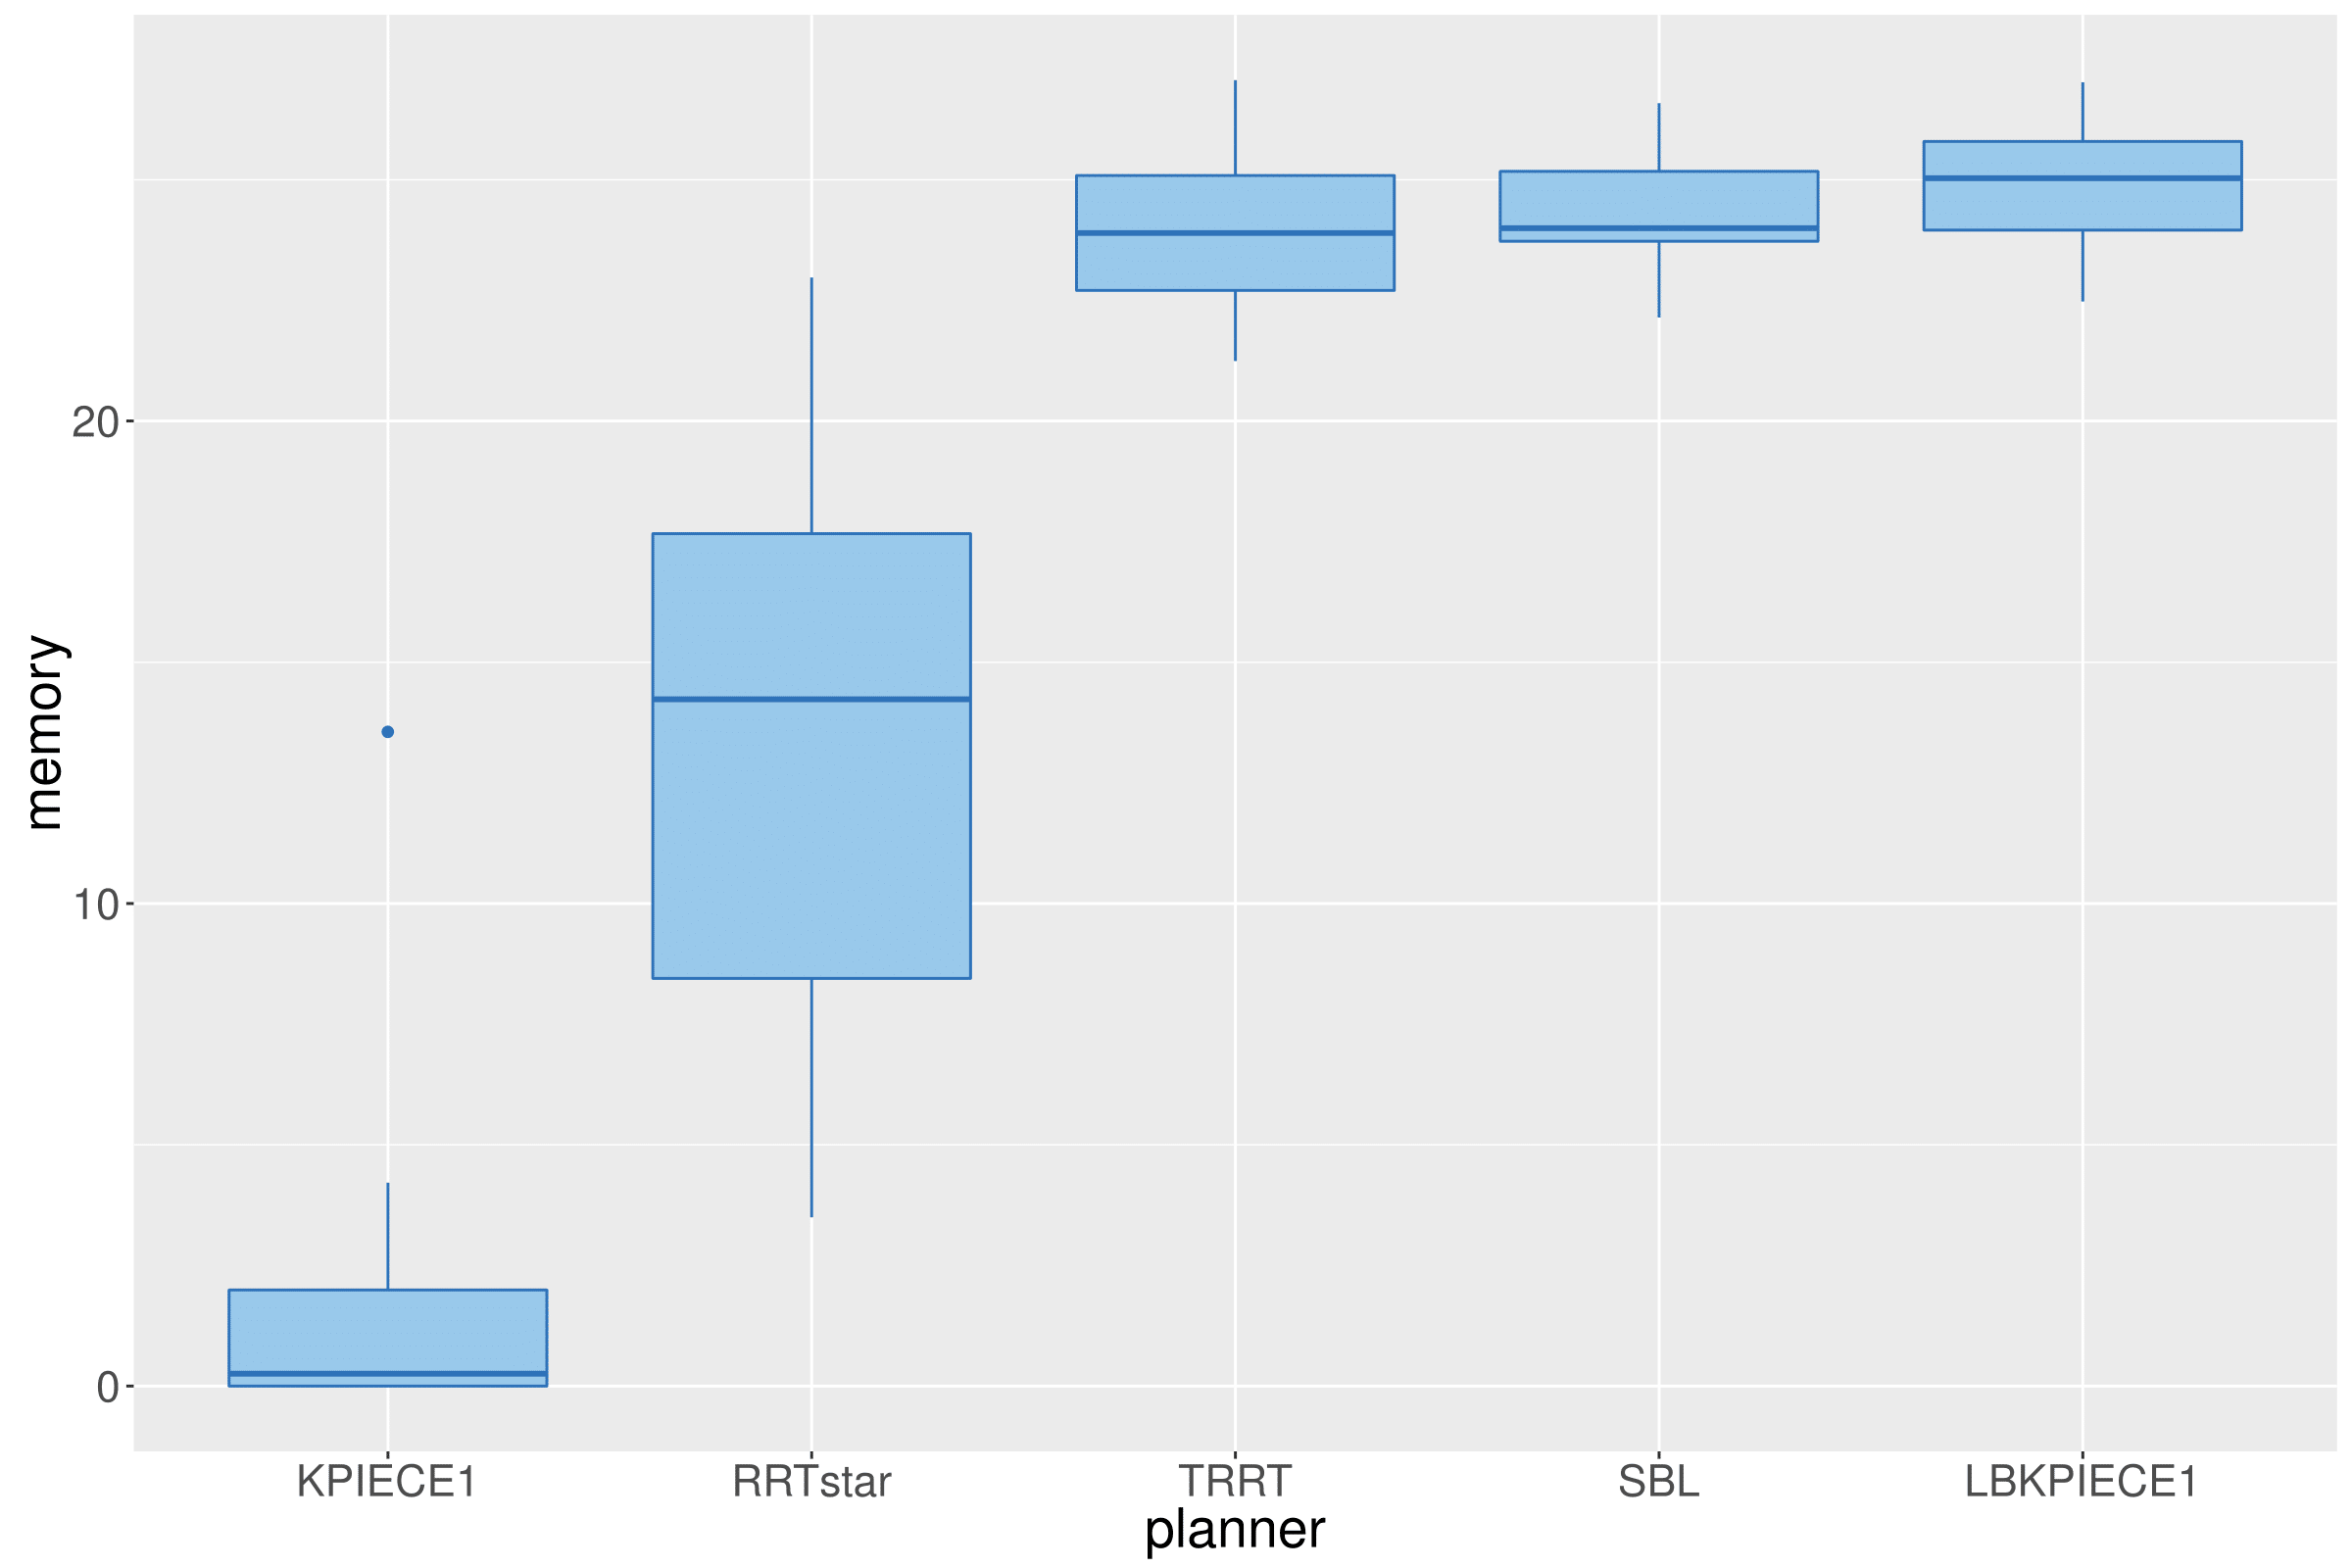
\includegraphics[width=0.8\textwidth,scale=0.6]{images/norm_memory-1.png}}
	\caption{Memory Consumption of Planners without Table Optimization}
	\label{fig:bm5}
\end{figure}
\begin{figure}[!ht] %  figure placement: here, top, bottom, or page
	\centering
	\frame{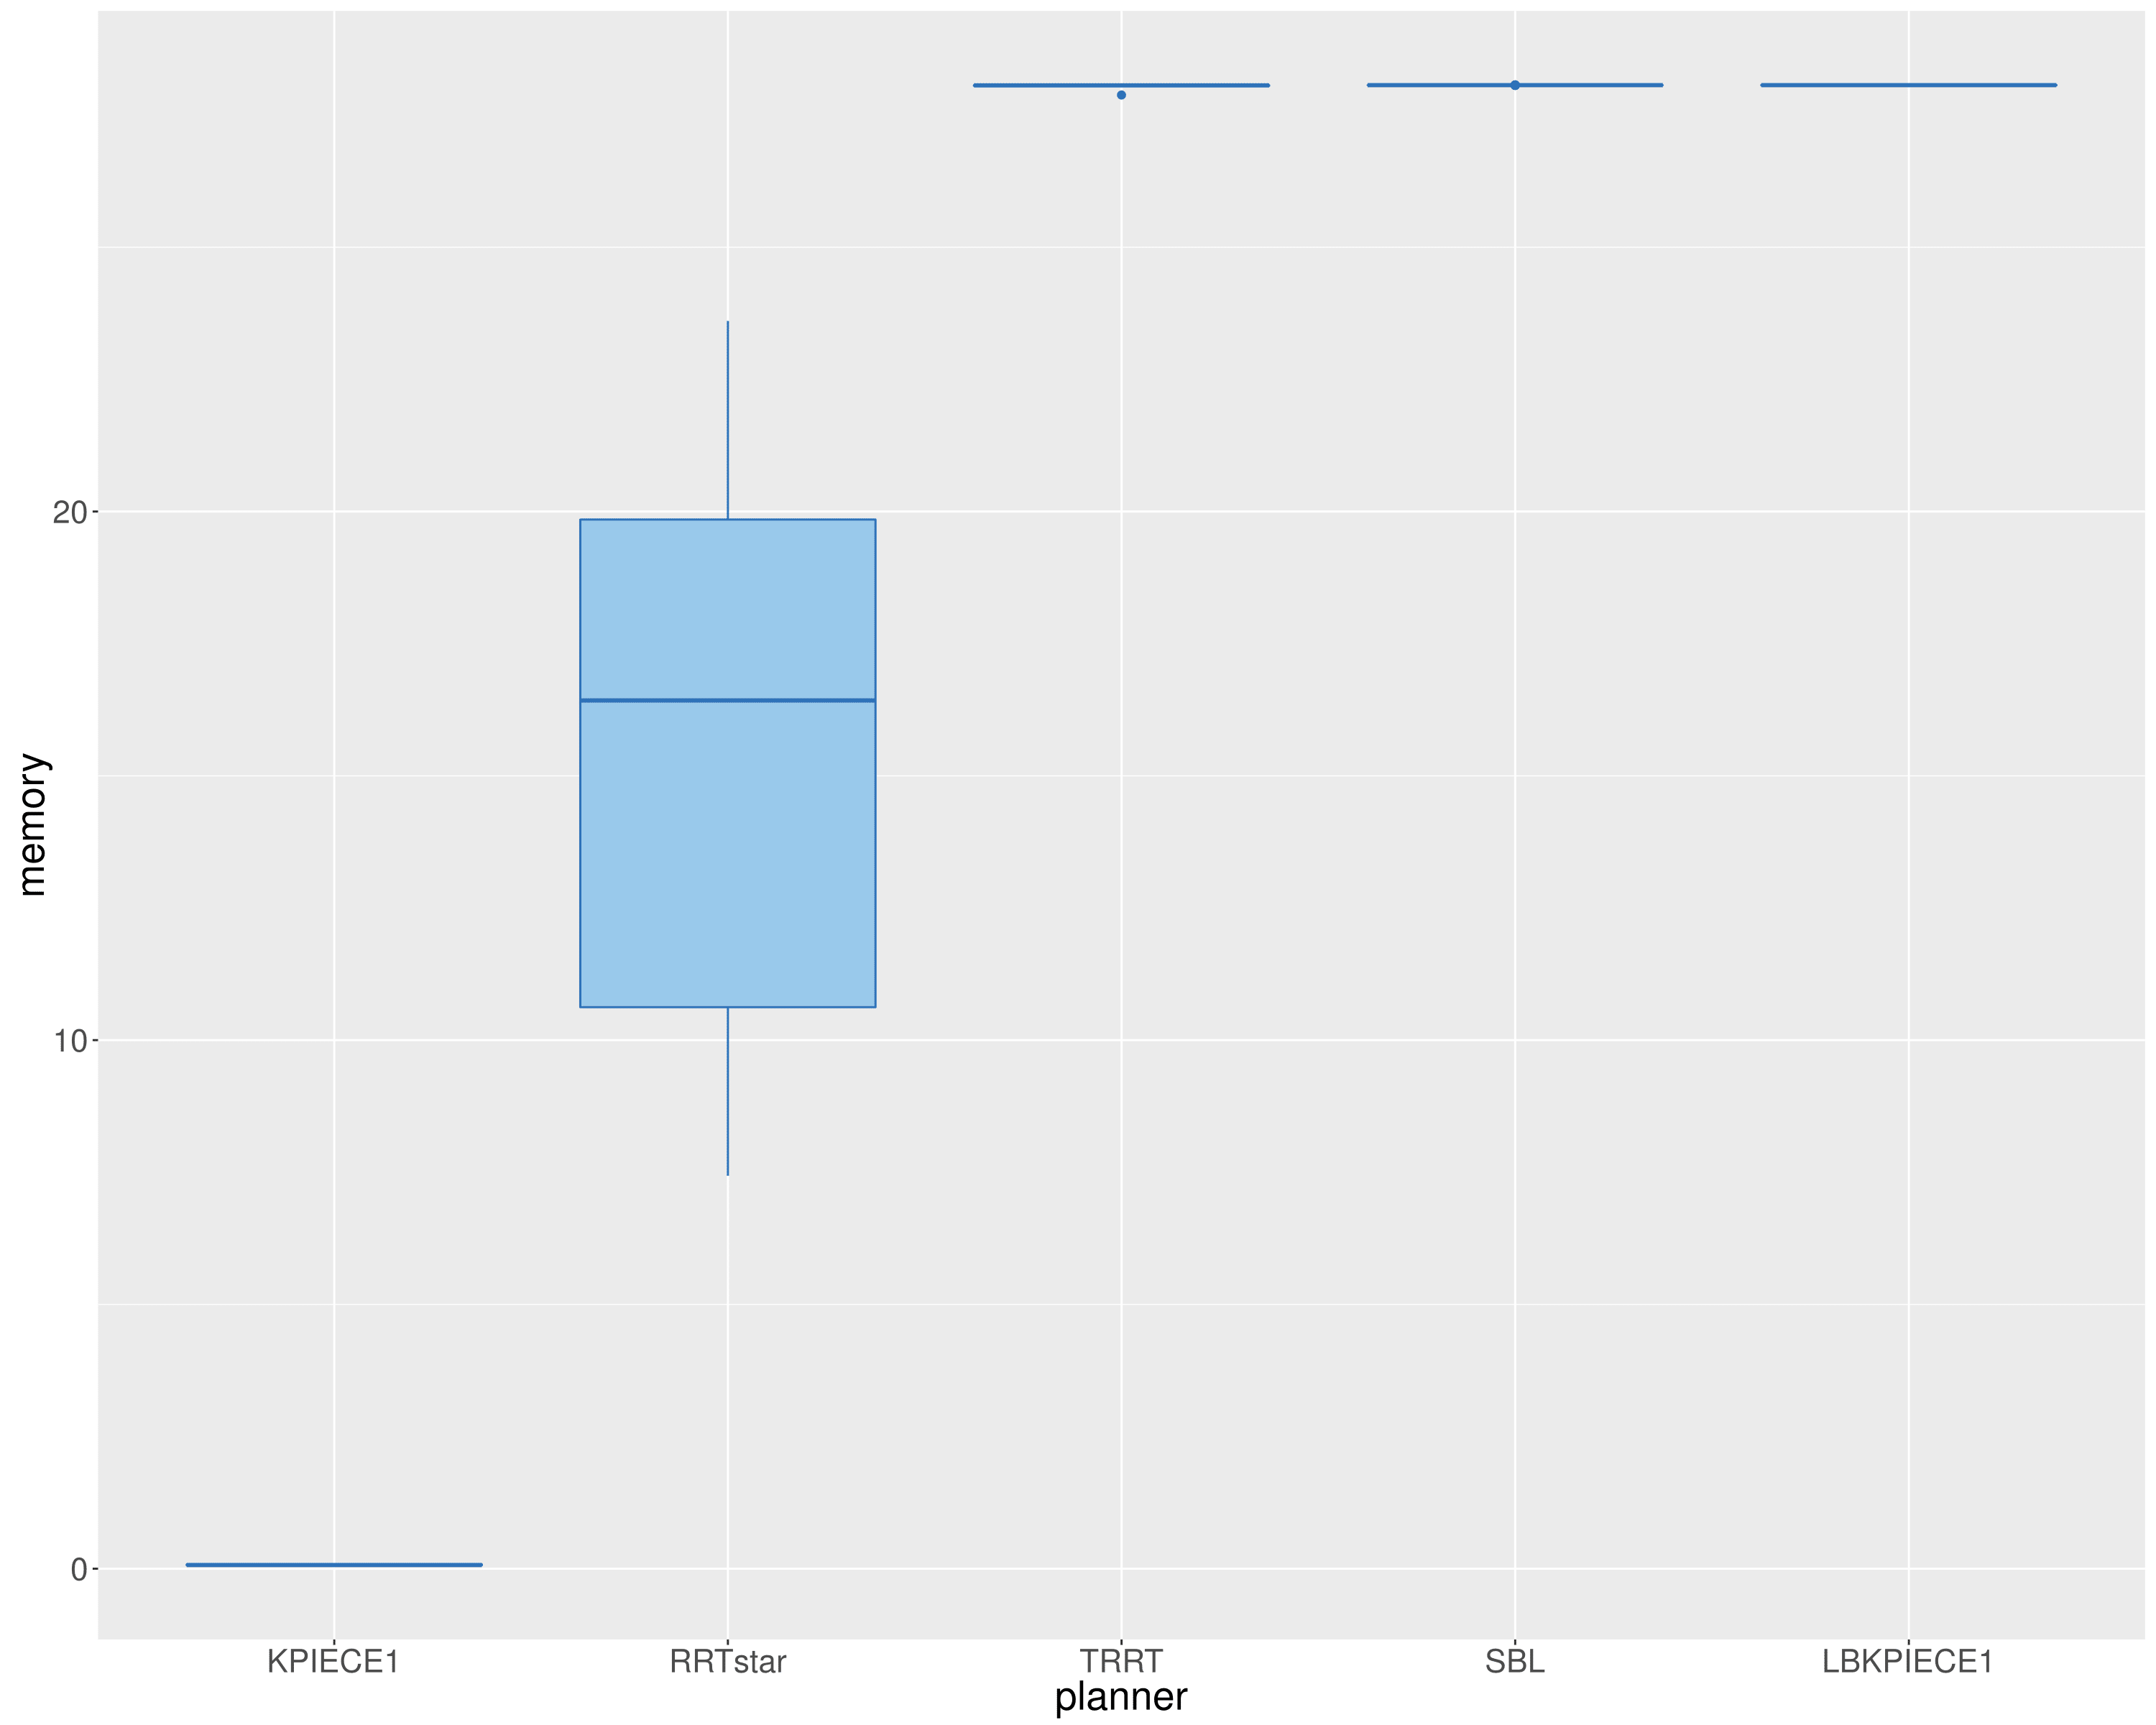
\includegraphics[width=0.8\textwidth,scale=0.6]{images/opt_memory-1.png}}
	\caption{Memory Consumption of Planners with Table Optimization }
	\label{fig:bm6}
\end{figure}
\begin{figure}[!ht] %  figure placement: here, top, bottom, or page
	\centering
	\frame{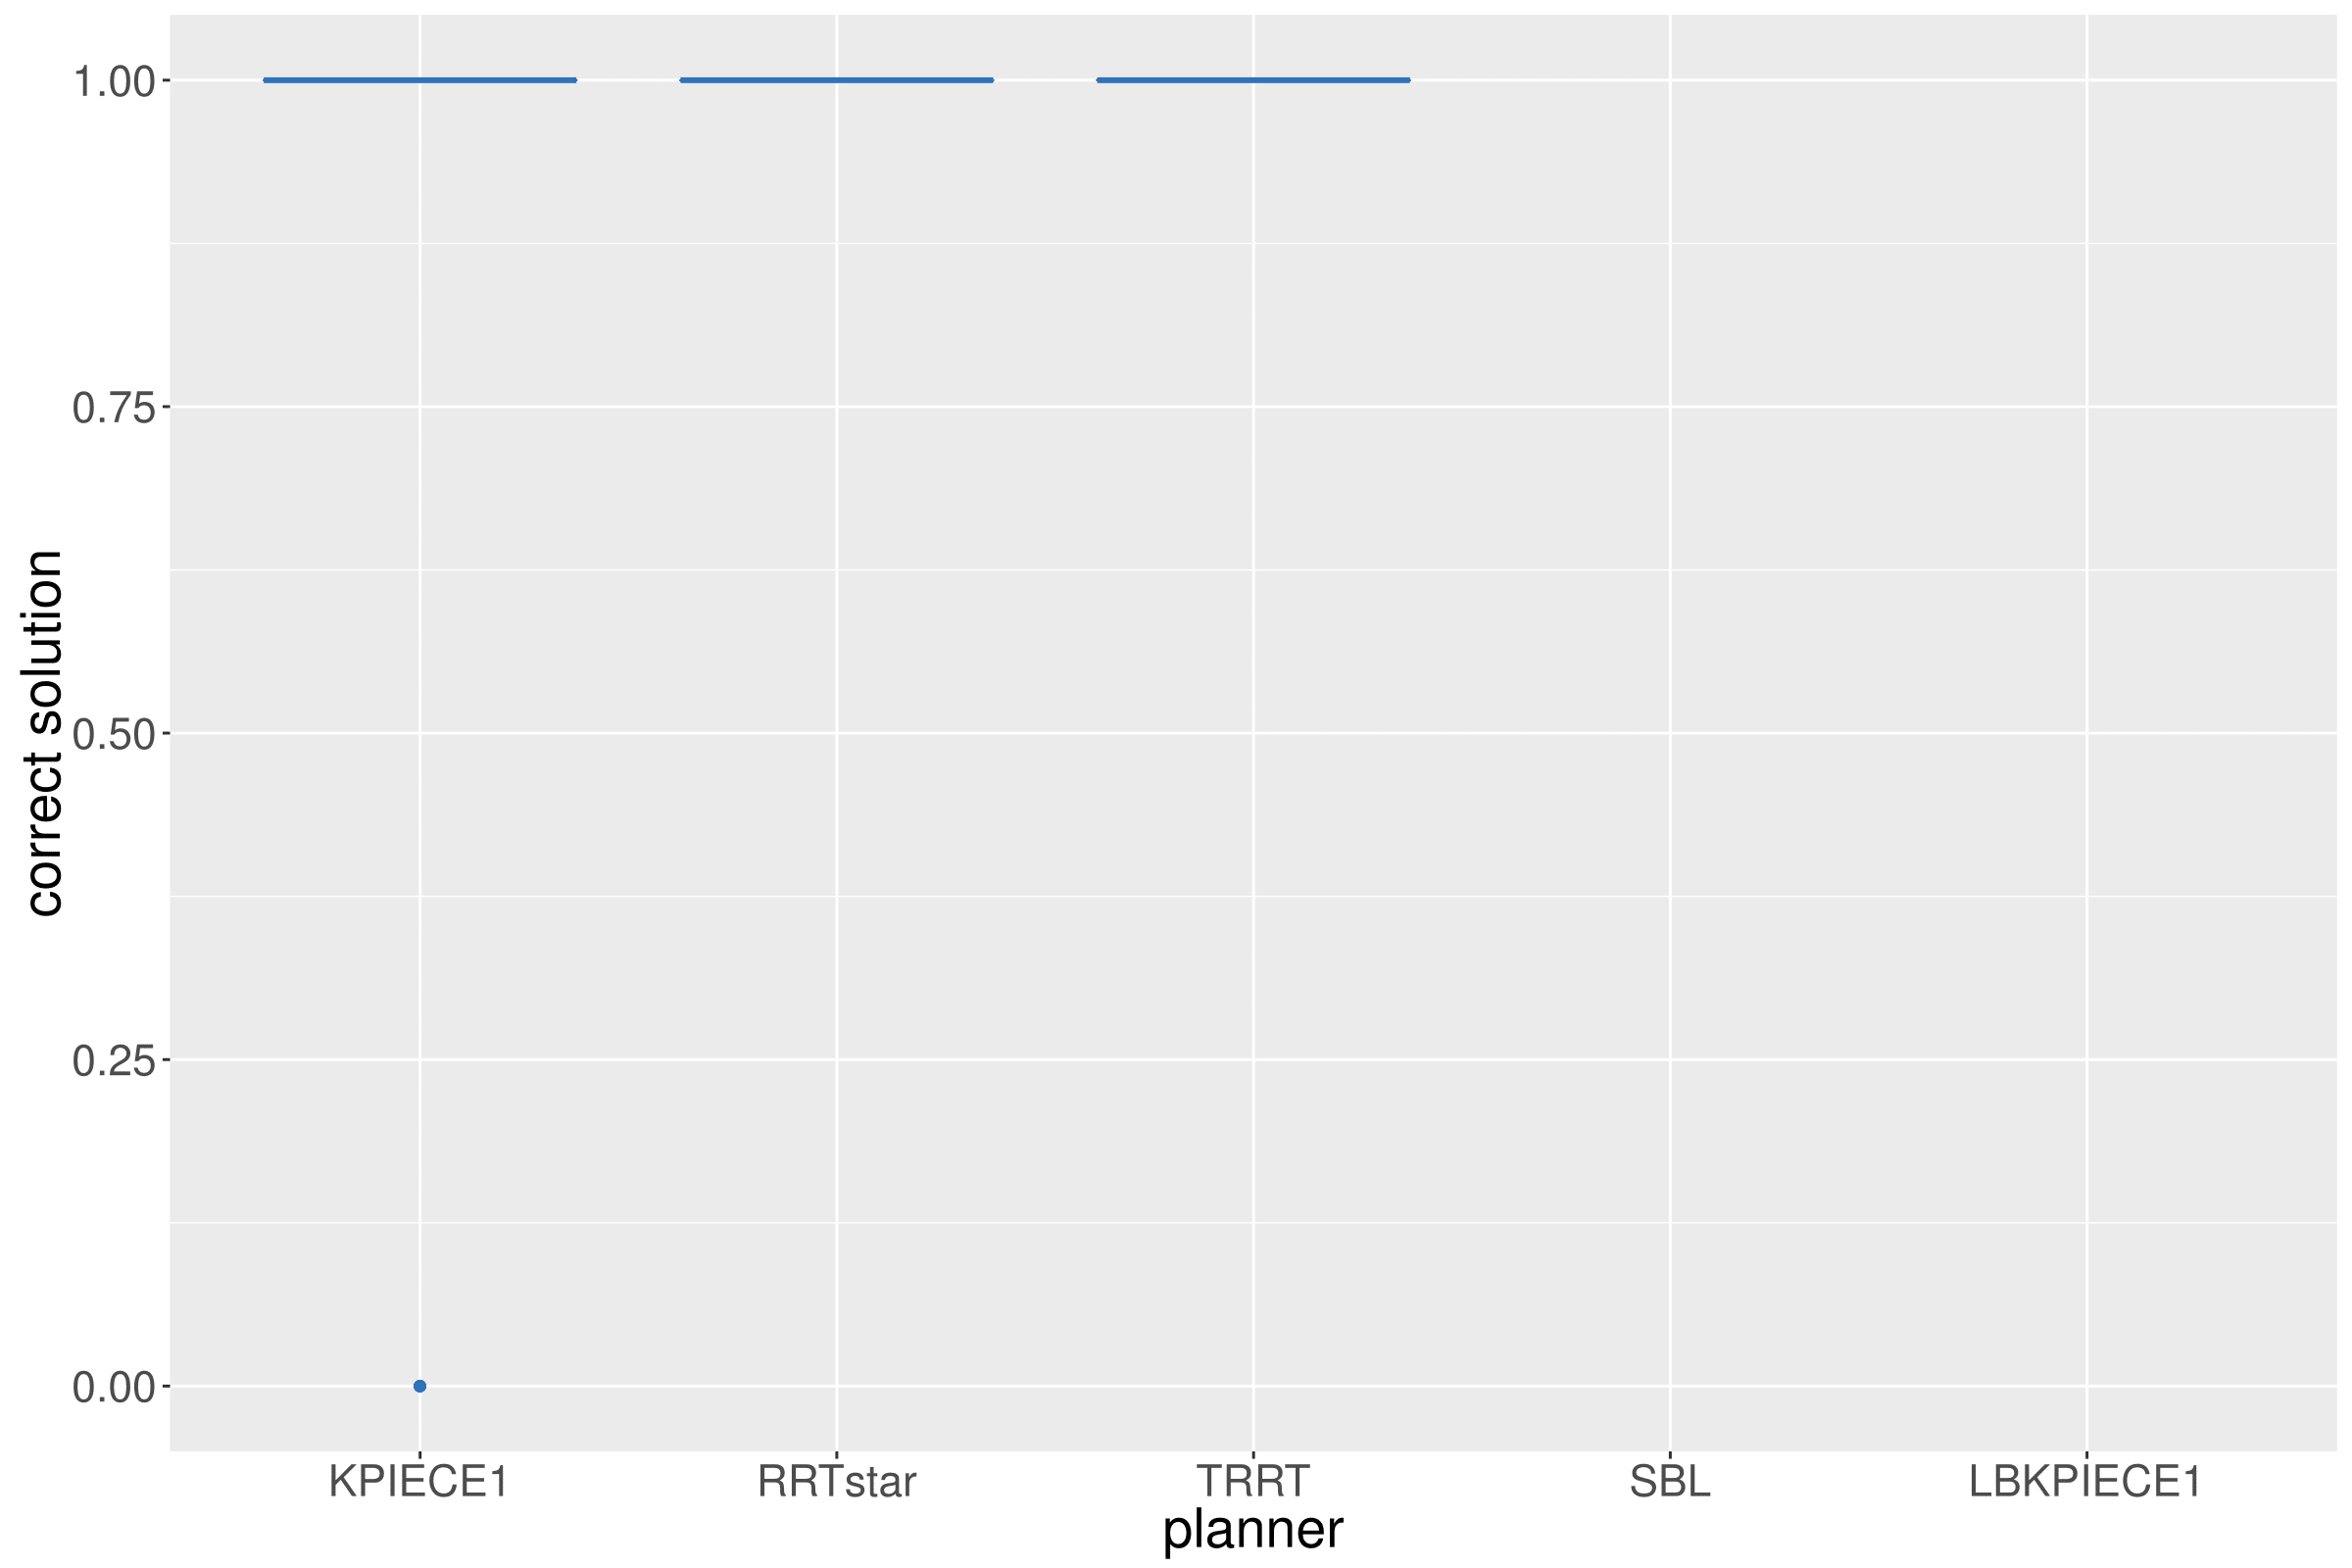
\includegraphics[width=0.8\textwidth,scale=0.6]{images/norm_corrsol-1.png}}
	\caption{Number of Correct Solutions Generated without Table Optimization}
	\label{fig:bm7}
\end{figure}
\begin{figure}[!ht] %  figure placement: here, top, bottom, or page
	\centering
	\frame{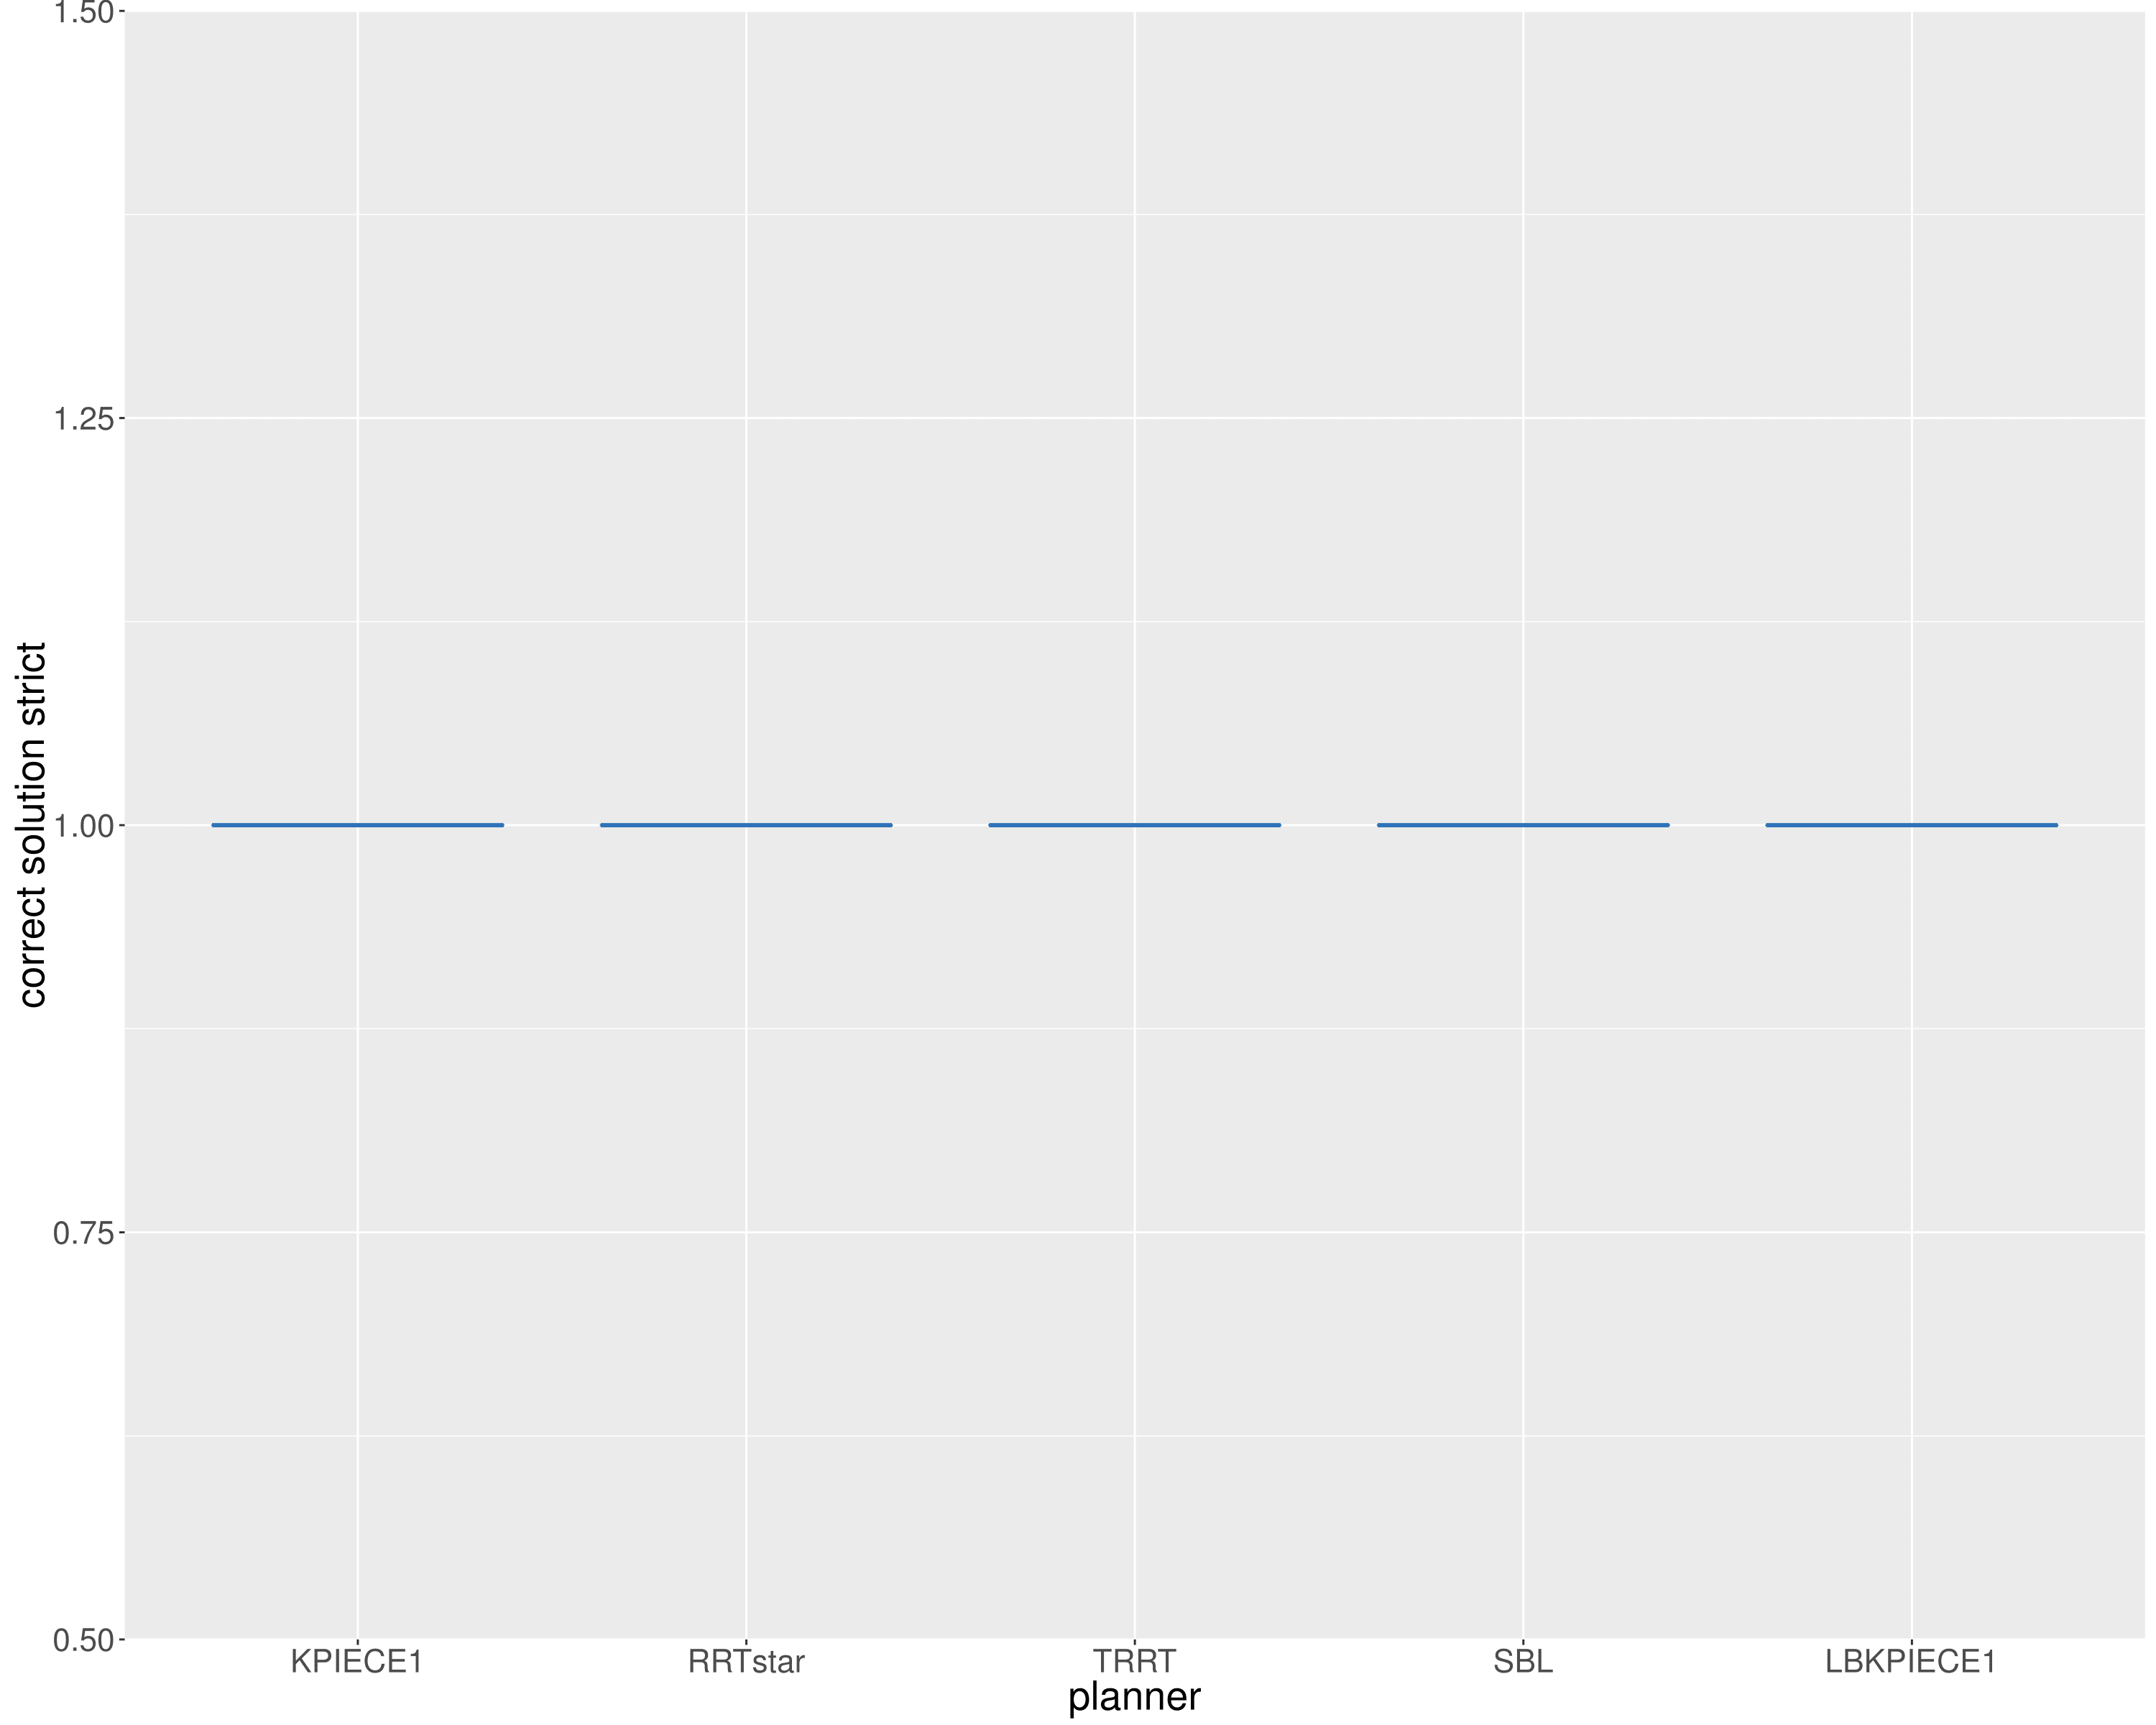
\includegraphics[width=0.8\textwidth,scale=0.6]{images/opt_corrsol-1.png}}
	\caption{Number of Correct Solutions Generated With Table Optimization}
	\label{fig:bm8}
\end{figure}
From the results its clear, the table optimization works.